\documentclass[a4paper]{article}
\usepackage[colorlinks,linkcolor=black,urlcolor=black]{hyperref}
\usepackage{float}
\usepackage{mhchem}
\usepackage{mathrsfs}
\usepackage{pdfpages}
\usepackage{listings}
\usepackage{enumerate}
\usepackage{amsmath}
\usepackage{amssymb}
\usepackage{graphicx}
\usepackage{subfigure}
\usepackage{siunitx}
\usepackage{wrapfig}
\usepackage{geometry}
\usepackage{indentfirst}
\usepackage{multirow} 
\setlength{\parindent}{2em}
\renewcommand{\baselinestretch}{1.6}
\usepackage[greek,english]{babel} 
%\renewcommand\thesection{\Roman{section}}
%\renewcommand\thesubsection{\Alph{subsection}}
\geometry{left=2.5cm,right=2.5cm,top=2.5cm,bottom=2.5cm}
\begin{document}
\begin{titlepage}
\begin{figure}[!htbp]
\center

\includegraphics[width=12cm]{ji_logo.png}
\end{figure}
\noindent\rule[0.25\baselineskip]{\textwidth}{1pt}
\begin{center}
\Large{\bfseries  VV285, Honors Mathematics III \\Project}
\vspace{1cm}

\Huge{\bfseries The Caustic in the Coffee Cup}

\vspace{1.5cm}

\Large SU2018  Group 23\\

\vspace{1cm}
\Large Group members\\

\begin{tabular}{l l}
Ma Ziqiao & 517370910114\\
Guan Kaiwen & 517021911143\\
Xu Kailun & 517370910177\\
Zhang Zhenyuan & 517370910124\\
Gao Yang & 516141910036\\
\end{tabular}

\vspace{2cm}
{\bfseries July 28, 2018}\\
\vspace{2cm}

UM-SJTU Joint Institute
\end{center}
\end{titlepage}
\section{Abstract}
The objective of this project is to understand and analyze the optical phenomenon about caustic in the coffee cup. We start our work from the theoretical stage. In this stage, we initially recall the reflection theorem of light and photon density as basic background of our project. By analyzing the envelop of the family of curves, we figure out the formation of a nephroid and cardioid. Based on these analysis we achieve the visibility of caustic finally in practical stage. Our visibility includes two parts. One part is achieved by software simulation and the other is a practical experiment.
    
    Based on the theoretical stage and practical stage, we figure out the formation of caustic in coffee cup and analyze this kind of optical phenomenon by applying mathematical method. Finally, we also prove this optical phenomenon by an experiment, which help us validate the formation of caustic better.

\newpage
\tableofcontents
\newpage
\listoffigures
\listoftables
\newpage
\section{Project Introduction}
In our life, many people enjoy drinking a cup of coffee every day. There is an interesting thing happened in the coffee cup that many people have once noticed. This thing is coffee cup caustic, which is always generated when a light shines into the coffee cup in a certain way. 

This caustic appeared in the coffee cup is a bright circle-like light ring with a cusp (see Figure \ref{fig:intro}). 

\begin{figure}[!htbp]
    \centering
    
\includegraphics[width=6cm]{intro.png}
    \caption{The Caustic in the Coffee Cup [1]}
    \label{fig:intro}
\end{figure} 

Actually it is a kind of optical phenomenon in physics. In optics field, caustic is the envelope of light reflected by a curved surface. Because of the curved surface, the envelope is concentrated with bright light edge. And there always be a cusp in the bright edge.

Our project is to analyse this kind of optical phenomenon and validate it by ourselves based on some physical principles and mathematical principle.

\section{Theoretic Background}
\subsection{The reflection theorem of light}
Usually the spectrum obey the reflection law in the propagating medium. Basically we can show the law in flat surface with the help of a mirror. 

\begin{figure}[!htbp]
    \centering
    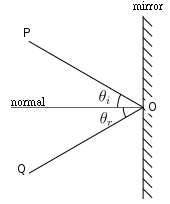
\includegraphics[width=6cm]{mirror.png}
    \caption{Diagram of light reflection [2]}
    \label{fig:mirror}
\end{figure}

In Figure \ref{fig:mirror}, $p$ is the source of the light ray , and $\overline{PO}$ is the incoming direction.  After the light ray reflects at the point $O$, the direction of light ray changes into $\overline{OQ}$. In this process, the angular between $\overline{PO}$ and normal  $\theta_i$ is equal to the angular between $\overline{OQ}$ and normal $\theta_r$, $st.$
$$ \theta_i=\theta_r $$
Therefore, the reflection law can be summarized as "angle of incidence" is equal to "angle of reflection".
\subsection{The relation between brightness and photon density}
Before the relation between brightness and photon density, we should know the theorem background of brightness and photon density.
\paragraph{Brightness}

Brightness is a visual perception, and it is a kind of way to express the strength of radiating ability and reflecting ability. Brightness is the perceptive stage of the luminance of a visual object. But brightness is not necessarily proportional to luminance. Because colour is also a key factor that can affect the brightness. In this project we mainly discuss the brightness with a specific colour, therefore, the brightness is mainly affected by the luminance.
\paragraph{Photon density}

Literally speaking, photon density is the number of photons placed in a specific area. It is indeed such a significance. Actually photon density has more important meaning than its definition. The luminance of a specified point of a specified light source can be defined as
    \begin{equation*}
        L_v=n^2\frac{\text{d}\Phi _v}{\text{d}G}
    \end{equation*}
    where $\text{d}G$ is the etendue of an infinitesimally narrow beam containing the specified ray. $\text{d}\Phi _v$ is the luminous flux carried by the beam. $n$ is the index of refraction of the medium [3].
    
Therefore, in the situation of our project, the luminance is proportional to the luminous flux carried by the beam. And the luminous flux is decided by the density of photon.
    
Therefore, the brightness is positive related with the photon density. When the density of photon becomes higher, the brightness becomes higher.
\section{A Family of Parametrized Curves}
\subsection{Objective}
The section is oriented to question i). The objective of this section is to introduce the concept of \textbf{Family of Curve} for further discussion. After the section, readers should be able to comprehend the concept and the notations of a family of parametrized curves. Readers will also be shown some illustrative figures to visualize the concept.
\subsection{Definition and Notations}
In Vy 285, Honors Mathematics III, we learned the concept of curves. Defined on a finite-dimensional vector space $V$ and an interval $I \subset \mathbb{R}$, a curve $\mathcal{C} \subset V$ is parametrized by a continuous, surjective, and locally injective map $\gamma: I \to \mathcal{C}$, which is named parametrization [1].

A family of curves is a set of curves, each of which is given by a function or parametrization in which one or more of the parameters is variable [2]. A family of curves can be denoted similarly as $\{\gamma(p,\cdot):p \in J \subset \mathbb{R}\}$. Namely, for every real number $p \in I$, the corresponding $\gamma(p,t)$, $t \in I \subset \mathbb{R}$ will define a curve in $\mathbb{R}^2$.
\subsection{An Illustrative Example}
Consider a family of parametrized circles in $\mathbb{R}^2$.
$$\gamma(p,t) = (p \cos t, p\sin t + 2p), t \in [0,2\pi), p>0$$
To visualize the set of curves, 20 members from the family is plotted as follows by using \texttt{Python} (Figure \ref{fig:family}).

\begin{figure}[!htbp]
	\centering
	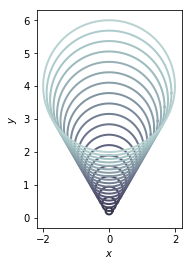
\includegraphics[width=0.4\textwidth]{family_20.png}
	\caption{20 Members from $\gamma(p,t) = (p \cos t, p\sin t + 2p), t \in [0,2\pi), p>0$}
	\label{fig:family}
\end{figure}

From the figure we observed that the members from the same family of curves have the following features.
\begin{itemize}
\item Although each member curve in a family is different in some details, they usually share a common appearance. As we can see in the figure, although different in terms of size and position, all the 20 members take on a circular shape.
\item For a continuous $\gamma$, the change of the appearance of adjacent members are continuous. From the figure we can see that the size and position changes in regular. There is no sudden change in the shape nor in the size for near $p$.
\item All the members in the graph occupy a limited region in the coordinate system. The members in the family don't span the whole $\mathbb{R}^2$, instead they are only present in a limited region (Figure \ref{fig:family_200}). 

\begin{figure}[!htbp]
	\centering
	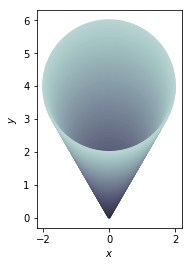
\includegraphics[width=0.4\textwidth]{family_200.png}
	\caption{200 Members from $\gamma(p,t) = (p \cos t, p\sin t + 2p), t \in [0,2\pi), p>0$}
	\label{fig:family_200}
\end{figure}
\end{itemize}

From the above discussion, we are now interested in the boundary of the region that the family of curves span. The concept of \textbf{envelop} will be introduced in the next section with respect to this concern.
\section{The Envelop of the Family of Curves}
\subsection{Objective}
The section is oriented to question ii). In the end of Section 4, we noticed a phenomenon that members of a family of parametrized curves are usually only present in some regions of the coordinate system. The objective of this section is to probe into the boundary of these regions and introduce the concept of \textbf{envelop} of a family of curves. The section will enable readers to comprehend the concept of an envelop of a family of parametrized curves, as will as understand how to find the envelop with the parametrization given. 
\subsection{Definition and Solution}
A curve that is tangent at every point to one of the curves $\gamma(p,\cdot)$ is called an envelope of the family of curves [4]. 

The later discussion is based on the following assumptions on the point of contact, where the envelop and a member curve intersect.
\begin{itemize}
\item The existence of the point of contact.

We discuss the problem on the interval $p \in J \subset \mathbb{R}$, where an arbitrary curve in this family is tangent to the curve, $i.e.$ for every $p$, there is some $\widetilde{t} \in I \subset \mathbb{R}$, such that $\gamma(p,\tilde{t})$ denotes the point of contact.
\item The local uniqueness of the point of contact.

The point of contact between a member curve and the envelop should be locally unique, $i.e.$, in some open ball $B_{\epsilon}(\tilde{t})$ around $\widetilde{t}$, the point of contact $\gamma(p,\tilde{t})$ is unique. This guarantees the existence of such a map 
$$h: J \supset B_{\sigma}(p) \to B_{\epsilon}(\tilde{t}) \subset \mathbb{R},\qquad\quad h(p)=\widetilde{t}$$
\end{itemize}

From the assumptions above we can conclude that, for every $p$ the point of contact can be denoted by $\gamma(p,h(p))$. Let $\psi: p \to (p,h(p))$. According to the definition of envelop, we find a parametrization of the envelop by
$$\gamma \circ \psi: J \to \mathcal{C},\qquad\quad \gamma \circ \psi (p) = \gamma(p,h(p))$$

Let $\gamma(p,t) = (\gamma_1(p,t),\gamma_2(p,t))$. The tangent vector of the envelop can be calculated by $T_{env}(p) = (\gamma \circ \psi)'(p)$. And by the chain rule we have
\begin{align*}
T_{env}(p) &= D\gamma \vert_{\psi(p)} \circ D\psi \vert_{p}\\
&= 
\begin{pmatrix}
\frac{\partial \gamma_1}{\partial p} & \frac{\partial \gamma_1}{\partial t}\\
\frac{\partial \gamma_2}{\partial p} & \frac{\partial \gamma_2}{\partial t}\\
\end{pmatrix}
\begin{pmatrix}
1\\
\frac{dh}{dp}\\
\end{pmatrix}\\
&=
\begin{pmatrix}
\frac{\partial \gamma_1}{\partial p} + \frac{\partial \gamma_1}{\partial t}\cdot \frac{dh}{dp}\\
\frac{\partial \gamma_2}{\partial p} + \frac{\partial \gamma_2}{\partial t}\cdot \frac{dh}{dp}\\
\end{pmatrix}
\end{align*}

The tangent vector of the curve $\gamma(p,t)$ can be calculated by
\begin{align*}
T_{cur}(t) &= D\gamma\vert_t\\
&=
\begin{pmatrix}
\frac{\partial \gamma_1}{\partial t}\\
\frac{\partial \gamma_2}{\partial t}\\
\end{pmatrix}\\
\end{align*}

The tangential vectors $T_{env}$ and $T_{cur}$ are linearly dependent. Therefore
\begin{align*}
\det
\begin{pmatrix}
T_{env} & T_{cur}\\
\end{pmatrix}
&= 0\\
\det
\begin{pmatrix}
\frac{\partial \gamma_1}{\partial p} + \frac{\partial \gamma_1}{\partial t}\cdot \frac{dh}{dp} & \frac{\partial \gamma_1}{\partial t}\\
\frac{\partial \gamma_2}{\partial p} + \frac{\partial \gamma_2}{\partial t}\cdot \frac{dh}{dp} & \frac{\partial \gamma_2}{\partial t}\\
\end{pmatrix}
&= 0\\
\frac{\partial \gamma_2}{\partial t}(\frac{\partial \gamma_1}{\partial p} + \frac{\partial \gamma_1}{\partial t}\cdot \frac{dh}{dp}) &= \frac{\partial \gamma_1}{\partial t}(\frac{\partial \gamma_2}{\partial p} + \frac{\partial \gamma_2}{\partial t}\cdot \frac{dh}{dp})\\
\frac{\partial \gamma_2}{\partial t}\frac{\partial \gamma_1}{\partial p} &= \frac{\partial \gamma_1}{\partial t}\frac{\partial \gamma_2}{\partial p}
\end{align*}

Therefore, we draw to a conclusion that by solving the equation 
$$\frac{\partial \gamma_1}{\partial p}\frac{\partial \gamma_2}{\partial t} = \frac{\partial \gamma_1}{\partial t}\frac{\partial \gamma_2}{\partial p},$$
we can find the envelop of a family of curves parametrized by $\gamma(p,\cdot)$.
\subsection{An Illustrative Example}
Now we are able to answer the original question. The envelop of the family of curves
$$\gamma(p,t) = (p \cos t, p\sin t + 2p), t \in [0,2\pi), p>0$$
considered in Section 4 can now be calculated.
\begin{align*}
\frac{\partial \gamma_1}{\partial p}\frac{\partial \gamma_2}{\partial t} &= \frac{\partial \gamma_1}{\partial t}\frac{\partial \gamma_2}{\partial p}\\
\cos t \cdot p\cos t &= -p \sin t\cdot(\sin t +2)\\
\sin t &= -\frac{1}{2}
\end{align*}
For $t \in [0,2\pi)$, the solution is $t = \frac{7}{6}\pi$ or $t = \frac{11}{6}\pi$. Plug this in the original parametrization $\gamma$, the parametrization of the envelop is
$$\gamma \circ \psi(p) = (-\frac{\sqrt{3}}{2}p,\frac{3}{2}p), \qquad\qquad p>0$$
or
$$\gamma \circ \psi(p) = (\frac{\sqrt{3}}{2}p,\frac{3}{2}p), \qquad\qquad p>0$$

Thus the envelop is given by $y = \sqrt{3}\vert x \vert$ (Figure \ref{fig:envelop}).

\begin{figure}[!htbp]
	\centering
	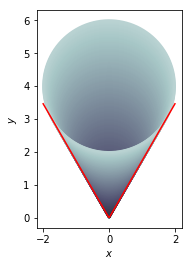
\includegraphics[width=0.4\textwidth]{family_200_envelop.png}
	\caption{200 Members from $\gamma(p,t) = (p \cos t, p\sin t + 2p), t \in [0,2\pi), p>0$, where the envelop of this family is coloured in red}
	\label{fig:envelop}
\end{figure}

From the above example, we would notice some features of an envelop.
\begin{itemize}
\item The envelop is tangential to all the curves in a family.
\item The envelop is the boundary of the region where the members of a family are present.
\item If the parametrization of a family is continuous, the envelop turn out to be a continuous (but not necessarily smooth) curve.
\item The envelop is the set containing all the intersection of members in a family that are infinitesimally close to each other.
\end{itemize}

The above are just visually observed conclusions, which remains to be verified.
\section{Discussion of the Catacaustic}
\subsection{Objective}
The section is oriented to question iii) and iv). The envelope of a reflected family of light rays is called a \textbf{catacaustic} [4]. The objective of this section is to apply the theoretic discussions into practice. We will go back to the caustic of a coffee cup, where the problem begins. After the section, readers should be able to understand how caustics are formed and will be shown how to find the parametrization of a caustic. In the following section, 2 examples of real situation of Catacaustics will be discussed: the Nephroid and the Cardioid.
\subsection{The Formation of a Nephroid}
\paragraph{Prerequisite Statement}
To form a Nephroid catacaustic curve, some prerequisite conditions must be satisfied.
\begin{itemize}
\item Nephroids are formed when parallel light rays (light source from infinity long distance) are reflected by a semi-circle [4].
\item The light beam will reflect in the semi-circle only once.
\end{itemize}

The following optical path will illustrate how the light beam travels and reflects in the semi-circle (Figure \ref{fig:optical path neph}).

\begin{figure}[!htbp] 
\centering 
\subfigure[The Optical Path]{
	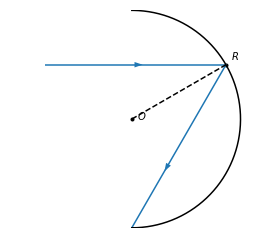
\includegraphics[width=0.5\linewidth]{opt_path_neph.png}  
	\label{fig:optical path neph} 
}
\subfigure[The Path in Coordinate (R = 1)]{
	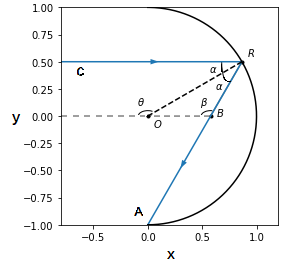
\includegraphics[width=0.5\linewidth]{opt_cor_neph.png} 
	\label{fig:optical coor neph} 
}
\caption{The Optical Illustration of a single Light Beam in a Nephroid} 
\end{figure}

\paragraph{Proof}
We set the path in a coordinate where the center of the semi-circle is placed at the origin and the light beam is parallel to the $x$-axis along the $+x$ direction. Assume the radius of the semi-circle to be $R$ (Figure \ref{fig:optical coor neph}).

We denote the angle between the the normal line where the reflection takes place and the $+x$-axis, $\angle ROx$, as $\theta$.

Since the light beam $AR$ is parallel to the $x$-axis, $\alpha + \theta = \pi$, so we have $\alpha = \pi - \theta$.

By the reflection theorem introduced in Section 3, $\angle ORC = \angle ORA = \alpha$. Consider the triangle $\Delta OBR$, $\theta = \alpha + \beta$, so we have $\beta = 2\theta - \pi$.

Therefore, the direction vector of the first order reflected light beam is given by $\lambda
\begin{pmatrix}
\cos (2\theta - \pi)\\
\sin (2\theta - \pi)\\
\end{pmatrix}$, which can be simplified as $\begin{pmatrix}
-\lambda \cos 2\theta\\
-\lambda \sin 2\theta
\end{pmatrix}$

The position of the reflection point $R$ is given by $\begin{pmatrix}
R \cos \theta\\
R \sin \theta\\
\end{pmatrix}$. Therefore, the for every $\theta$, the family of all reflection light beams is parametrized by
$$\gamma(\theta,\lambda) =
\begin{pmatrix}
R \cos \theta - \lambda \cos 2\theta\\
R \sin \theta - \lambda \sin 2\theta\\
\end{pmatrix}$$

According to the method introduced in Section 5, the envelop of the family of first order reflection curves can now be found by solving the differential equation:
\begin{align*}
\frac{\partial \gamma_1}{\partial \theta}\frac{\partial \gamma_2}{\partial \lambda} &= \frac{\partial \gamma_1}{\partial \lambda}\frac{\partial \gamma_2}{\partial \theta}\\
(-R\sin \theta + 2\lambda \sin 2\theta)(-\sin 2\theta) &= -\cos 2\theta (R\cos \theta - 2\lambda \cos 2\theta)\\
2\lambda \cos^2 2\theta + 2\lambda \sin^2 2\theta &= R \sin \theta \sin 2\theta + R \cos \theta \cos 2\theta\\
2\lambda &= R \cos (2\theta - \theta)\\
\lambda &= \frac{R}{2}\cos \theta
\end{align*}

Now we find the corresponding function that maps $\theta$ into $\lambda$. Plug this in the original parametrization $\gamma$, the parametrization of the envelop is
$$\gamma \circ \psi(\theta) =
\begin{pmatrix}
R\cos \theta - \frac{R}{2}\cos \theta \cos 2\theta\\
R\sin \theta - \frac{R}{2}\cos \theta \sin 2\theta\\
\end{pmatrix}$$

Note that in trigonometric calculation, we have the following formulae:
$$\sin 3\alpha = 3\sin \alpha - 4 \sin^3 \alpha$$
$$\cos 3\alpha = -3\cos \alpha + 4 \cos^3 \alpha$$

Consider the situation where $R=1$. Thus we have
\begin{align*}
\gamma_1(\theta) &= \cos \theta - \frac{1}{2}\cos \theta \cos 2\theta\\
&= \cos \theta - \frac{1}{2}\cos \theta (2\cos^2 \theta -1)\\
&= \frac{3}{2}\cos \theta - \cos^3 \theta\\
&= \frac{1}{4}\cos 3\theta -\frac{3}{4}\cos \theta + \frac{3}{2}\cos \theta\\
&= \frac{1}{4}(3\cos \theta - \cos 3\theta)
\end{align*}
\begin{align*}
\gamma_2(\theta) &= \sin \theta - \frac{1}{2}\cos \theta \sin 2\theta\\
&= \sin \theta - \frac{1}{2}\cos \theta (2\sin \theta \cos \theta)\\
&= \sin \theta - \sin \theta \cos^2 \theta\\
&= \sin^3 \theta\\
&= \frac{1}{4}(3\sin \theta - \sin 3\theta)
\end{align*}

Then we have a simplified version of the parametrization of the envelop
$$\gamma \circ \psi(\theta) = \frac{1}{4}
\begin{pmatrix}
3\cos \theta - \cos 3\theta\\
3\sin \theta - \sin 3\theta\\
\end{pmatrix}$$

Replace $\theta$ by $t$ and we get the parametric equations:
\begin{equation*}
\left\lbrace
	\begin{aligned}
	x = \frac{1}{4}(3\cos t - \cos 3t)\\
	y = \frac{1}{4}(3\sin t - \sin 3t)
	\end{aligned}
\right.
\end{equation*}

Note that the geometric meaning of $t$ is the angle $\theta$, the angle between the the normal line where the reflection takes place and the $+x$-axis. Thus the suitable range of $t$ is given by 
$$t \in [\frac{\pi}{2},\frac{3\pi}{2}].$$

\paragraph{Result Illustration}
The following is a theoretic display of the Nephroid (Figure \ref{fig:nephroid}). The figure is plotted by \texttt{Python}, assuming a semi-circle of $R=1$ and the parallel light beam from $-x$ axis to $+x$ axis.

\begin{figure}[!htbp]
	\centering
	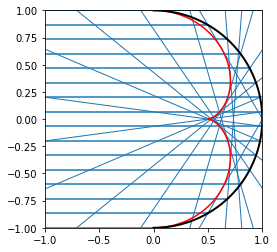
\includegraphics[width=0.6\textwidth]{nephroid.png}
	\caption{A Theoretic Display of a Nephroid, Denoted in Red Curve}
	\label{fig:nephroid}
\end{figure}

We observe a continuous, but not smooth curve in the graph. The non-differentiable point happens to be the intersection of several first order reflected light beams.
\subsection{The Formation of a Cardioid}
\paragraph{Prerequisite Statement}
Now we would like to probe into the curve observed in the coffee cup. To form a Cardioid catacaustic curve, some prerequisite conditions must be satisfied too.
\begin{itemize}
\item Cardioids are formed when the light source is directly above the rim of the cup, so that the light rays emanate from a point on the circle [4].
\item The light beam will reflect in the cup only once.
\end{itemize}

How the light beam travels and reflects in the cup is a a bit more complicated, but similar in principle (Figure \ref{fig:optical path card}).

\begin{figure}[!htbp] 
\centering 
\subfigure[The Optical Path]{
	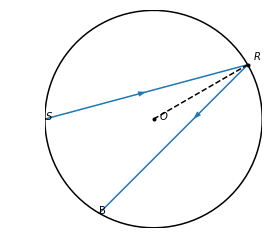
\includegraphics[width=0.5\linewidth]{opt_path_card.png}  
	\label{fig:optical path card} 
}
\subfigure[The Path in Coordinate (R = 1)]{
	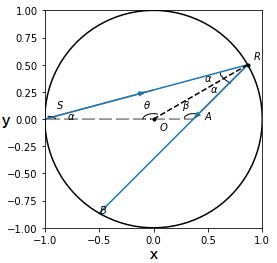
\includegraphics[width=0.5\linewidth]{opt_cor_card.png} 
	\label{fig:optical coor card} 
}
\caption{The Optical Illustration of a single Light Beam in a Cardioid} 
\end{figure}

\paragraph{Proof}
Assume the radius of the semi-circle to be $R$. Similar to the previous discussion about a nephroid, we set the path in a coordinate where the center of the cup is placed at the origin and the light source $S$ is set in the left side of the circle at $(-R,0)$(Figure \ref{fig:optical coor card}).

The parameter angle $\theta$ is also to be defined. We denote the angle between the the normal line where the reflection takes place and the $-x$-axis, $\angle ROx$, as $\theta$. And now we are prepared to start our proof.

Consider the triangle $\Delta OSR$, where $\overline{OS} = \overline{OR} = R$. We have $\angle OSR =\angle ORS = \alpha$. Since $\alpha+\alpha+\theta = \pi$, we have $\alpha = \frac{1}{2}(\pi-\theta)$.

Consider the reflection point $R$. By the reflection theorem, $\angle ORS = \angle ORB = \alpha$.

Now we consider the triangle $\Delta OAR$. Since $\theta = \beta +\alpha$, we find
\begin{align*}
\beta &= \theta - \alpha\\
&= \theta - \frac{1}{2}(\pi-\theta)\\
&=\frac{3}{2}\theta-\frac{\pi}{2}
\end{align*}

Therefore, the direction vector of the first order reflected light beam in a cup is given by $\lambda
\begin{pmatrix}
\cos (\beta)\\
\sin (\beta)\\
\end{pmatrix}$. Plug in the previous calculation and simplify the equation to get $\begin{pmatrix}
-\lambda \sin \frac{3}{2}\theta\\
\lambda \cos \frac{3}{2}\theta
\end{pmatrix}$

The position of the reflection point $R$ is again given by $\begin{pmatrix}
R \cos \theta\\
R \sin \theta\\
\end{pmatrix}$. Consequently, for every $\theta$, the family of all reflection light beams is parametrized by
$$\gamma(\theta,\lambda) =
\begin{pmatrix}
R \cos \theta - \lambda \sin \frac{3}{2}\theta\\
R \sin \theta + \lambda \cos \frac{3}{2}\theta\\
\end{pmatrix}$$

Again, we solving the differential equations to find the envelop:
\begin{align*}
\frac{\partial \gamma_1}{\partial \theta}\frac{\partial \gamma_2}{\partial \lambda} &= \frac{\partial \gamma_1}{\partial \lambda}\frac{\partial \gamma_2}{\partial \theta}\\
(-R\sin \theta - \frac{3}{2}\lambda \cos \frac{3}{2}\theta)\cos \frac{3}{2}\theta &= -\sin \frac{3}{2}\theta (R\cos \theta - \frac{3}{2}\lambda \sin \frac{3}{2}\theta)\\
\frac{3}{2}\lambda \cos^2 \frac{3}{2}\theta + \frac{3}{2}\lambda \sin^2 \frac{3}{2}\theta &= -R \sin \theta \cos \frac{3}{2}\theta + R \cos \theta \sin \frac{3}{2}\theta\\
\frac{3}{2}\lambda &= R\sin (\frac{2}{3} \theta - \theta)\\
\lambda &= \frac{2R}{3}\cos \frac{\theta}{2}
\end{align*}

Now we find the corresponding function that maps $\theta$ into $\lambda$. Plug this in the original parametrization $\gamma$, the parametrization of the envelop is
$$\gamma \circ \psi(\theta) =
\begin{pmatrix}
R\cos \theta - \frac{2R}{3}\cos \frac{\theta}{2} \sin \frac{3}{2}\theta\\
R\sin \theta + \frac{2R}{3}\cos \frac{\theta}{2} \cos \frac{3}{2}\theta\\
\end{pmatrix}$$

Note that in trigonometric calculation, we have the Prosthaphaeresis Formulae:
$$\cos \alpha \sin \beta = \frac{1}{2}[\sin (\alpha+\beta)-\sin(\alpha-\beta)]$$
$$\cos \alpha \cos \beta = \frac{1}{2}[\cos (\alpha+\beta)+\sin(\alpha-\beta)]$$

Consider the situation where $R=1$. Thus we have a simplified version of the parametrization of the envelop
$$\gamma \circ \psi(\theta) = \frac{1}{4}
\begin{pmatrix}
\frac{2}{3}\cos \theta (1+\cos \theta)-\frac{1}{3}\\
\frac{2}{3}\sin \theta (1+\sin \theta)\\
\end{pmatrix}$$

Replace $\theta$ by $t$ and we get the parametric equations:
\begin{equation*}
\left\lbrace
	\begin{aligned}
	x = \frac{2}{3}\cos t (1+\cos t)-\frac{1}{3}\\
	y = \frac{2}{3}\sin t (1+\cos t)
	\end{aligned}
\right.
\end{equation*}

Note that the geometric meaning of $t$ is the angle $\theta$, the angle between the the normal line where the reflection takes place and the $-x$-axis. Thus the suitable range of $t$ is given by 
$$t \in [0,2\pi).$$

\paragraph{Result Illustration}
The following is a theoretic display of the Cardioid (Figure \ref{fig:cardioid}). The figure is plotted by \texttt{Python}, assuming a semi-circle of $R=1$ and the parallel light beam from $-x$ axis to $+x$ axis.

\begin{figure}[!htbp]
	\centering
	\includegraphics[width=0.6\textwidth]{cardioid.png}
	\caption{A Theoretic Display of a Cardioid, Denoted in Red Curve}
	\label{fig:cardioid}
\end{figure}

We again observe a continuous, but not smooth curve in the graph.
\section{The Visibility of the Caustic}
To find a representation of the density of photons, we first note that if a group of light rays are close enough to each other, we can treat them as parallel. This is due to the continuity of the map $\gamma$, so that the tangent vector at around a point can be arbitrarily close to each other.

Now, if we consider a point A, which is the image of the set $(p_0,t_0)$, we are interested in the small area  around this point, namely $[p_0-\Delta p,p_0+\Delta p]\times[t_0-\Delta t,t_0+\Delta t]$, is mapped into.

We first fix p and consider the interval $[t_0-\Delta t,t_0+\Delta t]$. It's clear that it is  mapped to the points along the light ray corresponding to the unique p. Moreover, they compose a line segment, and if we recall the definition of curve length, its length can be approximated by $2\Delta t \left \| \dfrac{\partial \gamma}{\partial t}\bigg|_{p=p_0,t=t_0}\right \|$ since $\Delta t$ is small.

Now, if we fix t and consider p, similar results is obtained. So in general, these points make up a parallelogram with center at A (we have just shown that locally, these light rays can be treated as parallel), whose neighbouring edges have length $2\Delta t \left \| \dfrac{\partial \gamma}{\partial t}\bigg|_{p=p_0,t=t_0}\right \|$ and $2\Delta p \left \| \dfrac{\partial \gamma}{\partial p}\bigg|_{p=p_0,t=t_0}\right \|$. The area of this parallelogram is the length of the two sides times the sine of the angle they form, call it $\theta$. 
$$ Area=4\Delta t \Delta p \left \| \dfrac{\partial \gamma}{\partial t}\bigg|_{p=p_0,t=t_0}\right \|   \left \| \dfrac{\partial \gamma}{\partial t}\bigg|_{p=p_0,t=t_0}\right \|\rm{sin}\theta=4\Delta t \Delta p\cdot \rm{det}J_\gamma $$
Since it is assumed that p denotes the light rays, t denotes the dots along the ray, and photons travel at constant speed, the total intensity of light is proportional to the area with respect to t and p. 
$$ Intensity \propto 2\Delta t\cdot 2\Delta p$$
Now, if we ignore the scaling coefficient of intensity, it follows clearly that the photon density can be represented as
$$ Density=\dfrac{Intensity}{Area}=\dfrac{1}{det\ J_\gamma}.$$
Which is simply the inverse of the determinant of the Jacobian of $\gamma$.
\section{Experiment Exploration of a Caustic}
\subsubsection{A Real Life Experiment}
The materials needed are as follows.
\begin{table}[!htbp]
    \centering
    \begin{tabular}{lc}
    \hline
    Devices or Materials&Quantity\\
    \hline
    piece of cloth&1\\
    coffee cup&1\\
    scissor&1\\
    pencil&1\\
    A4 paper&1\\
    LED light tube&1\\
    \hline
    \end{tabular}
    \caption{All devices used in the experiment}
\end{table}
    
\paragraph{Experiment Procedure}
\begin{enumerate}
        \item Use the piece of cloth to clear the inside of the coffee cup and ensure its internal surface smooth.
        
        \item Take out the A4 paper and put it on the the top of the coffee cup. Then use the pencil sketch a circle along the rim of the coffee cup.
        
        \item Cut this circle accurately with the scissor, then put this circular piece in the internal bottom of the coffee cup. (In this step, the circular piece of paper should be set flat and close to the bottom.)
        
        \item Take out the LED light tube and turn it on, then set the tube above the coffee cup.
        
        \item observe the circular paper inside of the cup. Meanwhile we keep adjusting the position of the LED tube until there is a clear caustic occurs in the circular paper.
    \end{enumerate}
    
\paragraph{Results Presentation}
    
    After finishing these steps above, we use a phone camera to record the result of our experiment. The experiment result is displayed as follows:
    
    \begin{figure}[!htbp]
        \centering
        \includegraphics[width=8cm]{caustic.jpg}
        \caption{Caustic Derived from Experiment}
        \label{fig:caustic}
    \end{figure}

\subsubsection{A Experiment Using Modelling Software}
The following experiment using a software may allow us to observe more possible situations. 

Rendered using Appleseed renderer in blender, which simulates photons reacting with different materials. The cylinder wall is in mirror material with reflection rate 1.0 and the bottom plane is rendered in diffuse material.

Assume the light source is above the cup and the its horizontal distance from the center of circle is set as $0,\frac{R}{4},\frac{R}{2},\frac{3R}{4},R$.

The results of different possible caustics are listed in the following figures.

    \begin{figure}[!htbp]
        \centering
        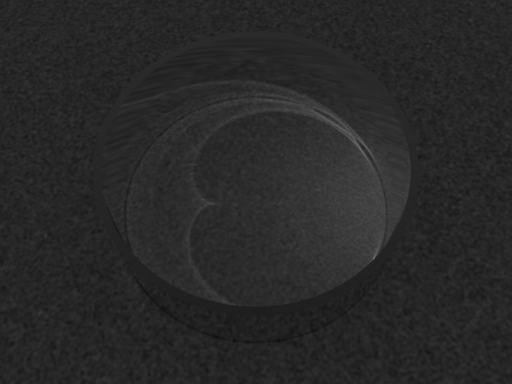
\includegraphics[width=10cm]{0001.png}
        \caption{Caustic Derived from Experiment, $d=R$}
        \label{fig:caustic}
    \end{figure}
    
       \begin{figure}[!htbp]
        \centering
        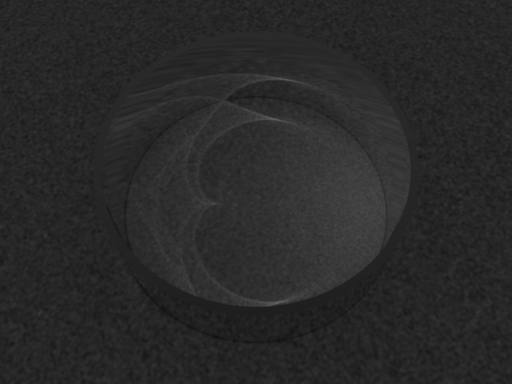
\includegraphics[width=10cm]{0002.png}
        \caption{Caustic Derived from Experiment, $d=\frac{3R}{4}$}
        \label{fig:caustic}
    \end{figure}
    
     \begin{figure}[!htbp]
        \centering
        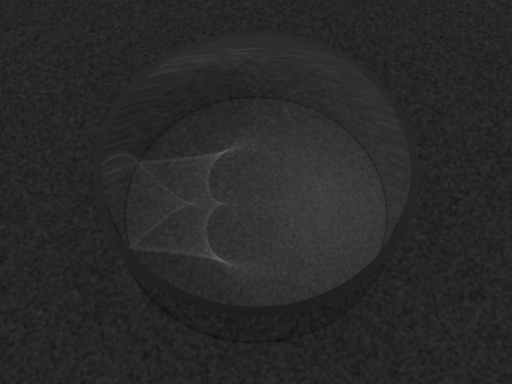
\includegraphics[width=10cm]{0003.png}
        \caption{Caustic Derived from Experiment, $d=\frac{R}{2}$}
        \label{fig:caustic}
    \end{figure}
    
      \begin{figure}[!htbp]
        \centering
        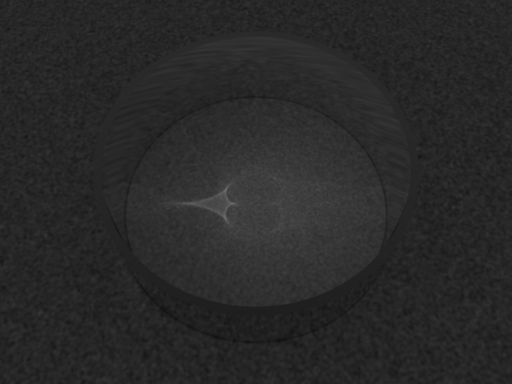
\includegraphics[width=10cm]{0004.png}
        \caption{Caustic Derived from Experiment, $d=\frac{R}{4}$}
        \label{fig:caustic}
    \end{figure}
    
      \begin{figure}[!htbp]
        \centering
        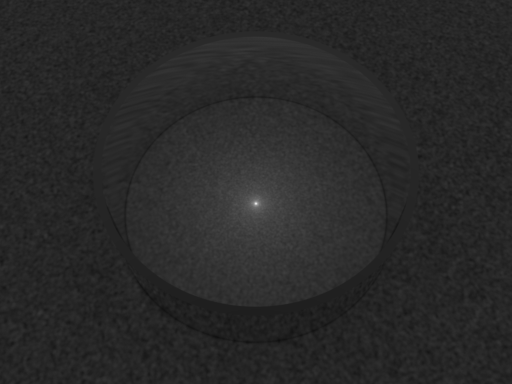
\includegraphics[width=10cm]{0005.png}
        \caption{Caustic Derived from Experiment,$d=0$}
        \label{fig:caustic}
    \end{figure}

\section{Conclusion}
In this project we explored the formation and the character of the caustic of coffee cup. During the process of exploring, we analyze it from theoretical stage to practical state. In the end we validate it by an experiment.

We began our analysis from a family of parametrized curves, which is the cornerstone of this project. Then we further analyze the envelop of the family of curve based on the a family of parametrized curves. Then we found that Nephroid and Cardioid are two key factors for caustic of coffee cup. Therefore, we respectively explore the formation of a Nephroid and the formation of a Cardioid. Finally we use some software to plot the caustic based on our exploration. 

Besides, we validated this interesting optical phenomenon practically by an experiment. During this process we found the position of light source can affect the caustic's shape and brightness directly.

In the future research, we may continue this topic and exploring it further by analyzing and finding the best position of light source for researchers to observe this phenomenon.

\section{References}
[1] “Caustics the envelope of light rays reflected,” FYPhysics. [Online]. Available: \url{http://fuckyeahphysica.tumblr.com/post/148153505356/ caustics-the-envelope-of-light-rays-reflected-or}

[2] “Reflection (physics),” Wekipedia. [Online]. Available: \url{https://en.wikipedia.org/ wiki/Reflection_(physics)#Laws of reflection}

[3] “Luminance,” Wekipedia. [Online]. Available: \url{https://en.wikipedia.org/wiki/ Luminance}

[4] H. Hohberger (2018). "vv285 main.pdf". UMJI-SJTU, Shanghai. Web. 31 Jul, 2018.

[5] "Family of a Curve." Wekipedia. [Online]. Available: \url{https://en.wikipedia.org/wiki/Family of curves}
\section{Appendix}
\subsection{\texttt{Python} Codes for the Figures}
This is one sample code for plotting. The rest are plotted similarly.
\lstset{language=C}
\begin{lstlisting}
\def\PY@reset{\let\PY@it=\relax \let\PY@bf=\relax%
    \let\PY@ul=\relax \let\PY@tc=\relax%
    \let\PY@bc=\relax \let\PY@ff=\relax}
\def\PY@tok#1{\csname PY@tok@#1\endcsname}
\def\PY@toks#1+{\ifx\relax#1\empty\else%
    \PY@tok{#1}\expandafter\PY@toks\fi}
\def\PY@do#1{\PY@bc{\PY@tc{\PY@ul{%
    \PY@it{\PY@bf{\PY@ff{#1}}}}}}}
\def\PY#1#2{\PY@reset\PY@toks#1+\relax+\PY@do{#2}}

\expandafter\def\csname PY@tok@w\endcsname{\def\PY@tc##1{\textcolor[rgb]{0.73,0.73,0.73}{##1}}}
\expandafter\def\csname PY@tok@c\endcsname{\let\PY@it=\textit\def\PY@tc##1{\textcolor[rgb]{0.25,0.50,0.50}{##1}}}
\expandafter\def\csname PY@tok@cp\endcsname{\def\PY@tc##1{\textcolor[rgb]{0.74,0.48,0.00}{##1}}}
\expandafter\def\csname PY@tok@k\endcsname{\let\PY@bf=\textbf\def\PY@tc##1{\textcolor[rgb]{0.00,0.50,0.00}{##1}}}
\expandafter\def\csname PY@tok@kp\endcsname{\def\PY@tc##1{\textcolor[rgb]{0.00,0.50,0.00}{##1}}}
\expandafter\def\csname PY@tok@kt\endcsname{\def\PY@tc##1{\textcolor[rgb]{0.69,0.00,0.25}{##1}}}
\expandafter\def\csname PY@tok@o\endcsname{\def\PY@tc##1{\textcolor[rgb]{0.40,0.40,0.40}{##1}}}
\expandafter\def\csname PY@tok@ow\endcsname{\let\PY@bf=\textbf\def\PY@tc##1{\textcolor[rgb]{0.67,0.13,1.00}{##1}}}
\expandafter\def\csname PY@tok@nb\endcsname{\def\PY@tc##1{\textcolor[rgb]{0.00,0.50,0.00}{##1}}}
\expandafter\def\csname PY@tok@nf\endcsname{\def\PY@tc##1{\textcolor[rgb]{0.00,0.00,1.00}{##1}}}
\expandafter\def\csname PY@tok@nc\endcsname{\let\PY@bf=\textbf\def\PY@tc##1{\textcolor[rgb]{0.00,0.00,1.00}{##1}}}
\expandafter\def\csname PY@tok@nn\endcsname{\let\PY@bf=\textbf\def\PY@tc##1{\textcolor[rgb]{0.00,0.00,1.00}{##1}}}
\expandafter\def\csname PY@tok@ne\endcsname{\let\PY@bf=\textbf\def\PY@tc##1{\textcolor[rgb]{0.82,0.25,0.23}{##1}}}
\expandafter\def\csname PY@tok@nv\endcsname{\def\PY@tc##1{\textcolor[rgb]{0.10,0.09,0.49}{##1}}}
\expandafter\def\csname PY@tok@no\endcsname{\def\PY@tc##1{\textcolor[rgb]{0.53,0.00,0.00}{##1}}}
\expandafter\def\csname PY@tok@nl\endcsname{\def\PY@tc##1{\textcolor[rgb]{0.63,0.63,0.00}{##1}}}
\expandafter\def\csname PY@tok@ni\endcsname{\let\PY@bf=\textbf\def\PY@tc##1{\textcolor[rgb]{0.60,0.60,0.60}{##1}}}
\expandafter\def\csname PY@tok@na\endcsname{\def\PY@tc##1{\textcolor[rgb]{0.49,0.56,0.16}{##1}}}
\expandafter\def\csname PY@tok@nt\endcsname{\let\PY@bf=\textbf\def\PY@tc##1{\textcolor[rgb]{0.00,0.50,0.00}{##1}}}
\expandafter\def\csname PY@tok@nd\endcsname{\def\PY@tc##1{\textcolor[rgb]{0.67,0.13,1.00}{##1}}}
\expandafter\def\csname PY@tok@s\endcsname{\def\PY@tc##1{\textcolor[rgb]{0.73,0.13,0.13}{##1}}}
\expandafter\def\csname PY@tok@sd\endcsname{\let\PY@it=\textit\def\PY@tc##1{\textcolor[rgb]{0.73,0.13,0.13}{##1}}}
\expandafter\def\csname PY@tok@si\endcsname{\let\PY@bf=\textbf\def\PY@tc##1{\textcolor[rgb]{0.73,0.40,0.53}{##1}}}
\expandafter\def\csname PY@tok@se\endcsname{\let\PY@bf=\textbf\def\PY@tc##1{\textcolor[rgb]{0.73,0.40,0.13}{##1}}}
\expandafter\def\csname PY@tok@sr\endcsname{\def\PY@tc##1{\textcolor[rgb]{0.73,0.40,0.53}{##1}}}
\expandafter\def\csname PY@tok@ss\endcsname{\def\PY@tc##1{\textcolor[rgb]{0.10,0.09,0.49}{##1}}}
\expandafter\def\csname PY@tok@sx\endcsname{\def\PY@tc##1{\textcolor[rgb]{0.00,0.50,0.00}{##1}}}
\expandafter\def\csname PY@tok@m\endcsname{\def\PY@tc##1{\textcolor[rgb]{0.40,0.40,0.40}{##1}}}
\expandafter\def\csname PY@tok@gh\endcsname{\let\PY@bf=\textbf\def\PY@tc##1{\textcolor[rgb]{0.00,0.00,0.50}{##1}}}
\expandafter\def\csname PY@tok@gu\endcsname{\let\PY@bf=\textbf\def\PY@tc##1{\textcolor[rgb]{0.50,0.00,0.50}{##1}}}
\expandafter\def\csname PY@tok@gd\endcsname{\def\PY@tc##1{\textcolor[rgb]{0.63,0.00,0.00}{##1}}}
\expandafter\def\csname PY@tok@gi\endcsname{\def\PY@tc##1{\textcolor[rgb]{0.00,0.63,0.00}{##1}}}
\expandafter\def\csname PY@tok@gr\endcsname{\def\PY@tc##1{\textcolor[rgb]{1.00,0.00,0.00}{##1}}}
\expandafter\def\csname PY@tok@ge\endcsname{\let\PY@it=\textit}
\expandafter\def\csname PY@tok@gs\endcsname{\let\PY@bf=\textbf}
\expandafter\def\csname PY@tok@gp\endcsname{\let\PY@bf=\textbf\def\PY@tc##1{\textcolor[rgb]{0.00,0.00,0.50}{##1}}}
\expandafter\def\csname PY@tok@go\endcsname{\def\PY@tc##1{\textcolor[rgb]{0.53,0.53,0.53}{##1}}}
\expandafter\def\csname PY@tok@gt\endcsname{\def\PY@tc##1{\textcolor[rgb]{0.00,0.27,0.87}{##1}}}
\expandafter\def\csname PY@tok@err\endcsname{\def\PY@bc##1{\setlength{\fboxsep}{0pt}\fcolorbox[rgb]{1.00,0.00,0.00}{1,1,1}{\strut ##1}}}
\expandafter\def\csname PY@tok@kc\endcsname{\let\PY@bf=\textbf\def\PY@tc##1{\textcolor[rgb]{0.00,0.50,0.00}{##1}}}
\expandafter\def\csname PY@tok@kd\endcsname{\let\PY@bf=\textbf\def\PY@tc##1{\textcolor[rgb]{0.00,0.50,0.00}{##1}}}
\expandafter\def\csname PY@tok@kn\endcsname{\let\PY@bf=\textbf\def\PY@tc##1{\textcolor[rgb]{0.00,0.50,0.00}{##1}}}
\expandafter\def\csname PY@tok@kr\endcsname{\let\PY@bf=\textbf\def\PY@tc##1{\textcolor[rgb]{0.00,0.50,0.00}{##1}}}
\expandafter\def\csname PY@tok@bp\endcsname{\def\PY@tc##1{\textcolor[rgb]{0.00,0.50,0.00}{##1}}}
\expandafter\def\csname PY@tok@fm\endcsname{\def\PY@tc##1{\textcolor[rgb]{0.00,0.00,1.00}{##1}}}
\expandafter\def\csname PY@tok@vc\endcsname{\def\PY@tc##1{\textcolor[rgb]{0.10,0.09,0.49}{##1}}}
\expandafter\def\csname PY@tok@vg\endcsname{\def\PY@tc##1{\textcolor[rgb]{0.10,0.09,0.49}{##1}}}
\expandafter\def\csname PY@tok@vi\endcsname{\def\PY@tc##1{\textcolor[rgb]{0.10,0.09,0.49}{##1}}}
\expandafter\def\csname PY@tok@vm\endcsname{\def\PY@tc##1{\textcolor[rgb]{0.10,0.09,0.49}{##1}}}
\expandafter\def\csname PY@tok@sa\endcsname{\def\PY@tc##1{\textcolor[rgb]{0.73,0.13,0.13}{##1}}}
\expandafter\def\csname PY@tok@sb\endcsname{\def\PY@tc##1{\textcolor[rgb]{0.73,0.13,0.13}{##1}}}
\expandafter\def\csname PY@tok@sc\endcsname{\def\PY@tc##1{\textcolor[rgb]{0.73,0.13,0.13}{##1}}}
\expandafter\def\csname PY@tok@dl\endcsname{\def\PY@tc##1{\textcolor[rgb]{0.73,0.13,0.13}{##1}}}
\expandafter\def\csname PY@tok@s2\endcsname{\def\PY@tc##1{\textcolor[rgb]{0.73,0.13,0.13}{##1}}}
\expandafter\def\csname PY@tok@sh\endcsname{\def\PY@tc##1{\textcolor[rgb]{0.73,0.13,0.13}{##1}}}
\expandafter\def\csname PY@tok@s1\endcsname{\def\PY@tc##1{\textcolor[rgb]{0.73,0.13,0.13}{##1}}}
\expandafter\def\csname PY@tok@mb\endcsname{\def\PY@tc##1{\textcolor[rgb]{0.40,0.40,0.40}{##1}}}
\expandafter\def\csname PY@tok@mf\endcsname{\def\PY@tc##1{\textcolor[rgb]{0.40,0.40,0.40}{##1}}}
\expandafter\def\csname PY@tok@mh\endcsname{\def\PY@tc##1{\textcolor[rgb]{0.40,0.40,0.40}{##1}}}
\expandafter\def\csname PY@tok@mi\endcsname{\def\PY@tc##1{\textcolor[rgb]{0.40,0.40,0.40}{##1}}}
\expandafter\def\csname PY@tok@il\endcsname{\def\PY@tc##1{\textcolor[rgb]{0.40,0.40,0.40}{##1}}}
\expandafter\def\csname PY@tok@mo\endcsname{\def\PY@tc##1{\textcolor[rgb]{0.40,0.40,0.40}{##1}}}
\expandafter\def\csname PY@tok@ch\endcsname{\let\PY@it=\textit\def\PY@tc##1{\textcolor[rgb]{0.25,0.50,0.50}{##1}}}
\expandafter\def\csname PY@tok@cm\endcsname{\let\PY@it=\textit\def\PY@tc##1{\textcolor[rgb]{0.25,0.50,0.50}{##1}}}
\expandafter\def\csname PY@tok@cpf\endcsname{\let\PY@it=\textit\def\PY@tc##1{\textcolor[rgb]{0.25,0.50,0.50}{##1}}}
\expandafter\def\csname PY@tok@c1\endcsname{\let\PY@it=\textit\def\PY@tc##1{\textcolor[rgb]{0.25,0.50,0.50}{##1}}}
\expandafter\def\csname PY@tok@cs\endcsname{\let\PY@it=\textit\def\PY@tc##1{\textcolor[rgb]{0.25,0.50,0.50}{##1}}}

\def\PYZbs{\char`\\}
\def\PYZus{\char`\_}
\def\PYZob{\char`\{}
\def\PYZcb{\char`\}}
\def\PYZca{\char`\^}
\def\PYZam{\char`\&}
\def\PYZlt{\char`\<}
\def\PYZgt{\char`\>}
\def\PYZsh{\char`\#}
\def\PYZpc{\char`\%}
\def\PYZdl{\char`\$}
\def\PYZhy{\char`\-}
\def\PYZsq{\char`\'}
\def\PYZdq{\char`\"}
\def\PYZti{\char`\~}
% for compatibility with earlier versions
\def\PYZat{@}
\def\PYZlb{[}
\def\PYZrb{]}
\makeatother


    % Exact colors from NB
    \definecolor{incolor}{rgb}{0.0, 0.0, 0.5}
    \definecolor{outcolor}{rgb}{0.545, 0.0, 0.0}



    
    % Prevent overflowing lines due to hard-to-break entities
    \sloppy 
    % Setup hyperref package
    \hypersetup{
      breaklinks=true,  % so long urls are correctly broken across lines
      colorlinks=true,
      urlcolor=urlcolor,
      linkcolor=linkcolor,
      citecolor=citecolor,
      }
    % Slightly bigger margins than the latex defaults
\end{lstlisting}
\end{document}
